\sect{Endliche Automaten}

\ssect{DEA}

Ein \textbf{deterministischer endlicher Automat} ist ein 5-Tupel
$M = (Q, \Sigma, \delta, q_0, F)$ mit
\begin{itemize}
    \item Menge von \textbf{Zustände} $Q = \{ q_0, \dots, q_n\}$
    \item \textbf{Eingabealphabet} $\Sigma = \{a_1, \dots, a_m\}$
    \item \textcolor{blue}{\textbf{Übergangsfunktion $\delta$}}: $Q \times \Sigma \rightarrow Q$
    \item \textbf{Startzustand} $q_0 \in Q$
    \item Menge \textcolor{Green}{\textbf{akzept. Zustände} $F$} $\subseteq Q$
\end{itemize}

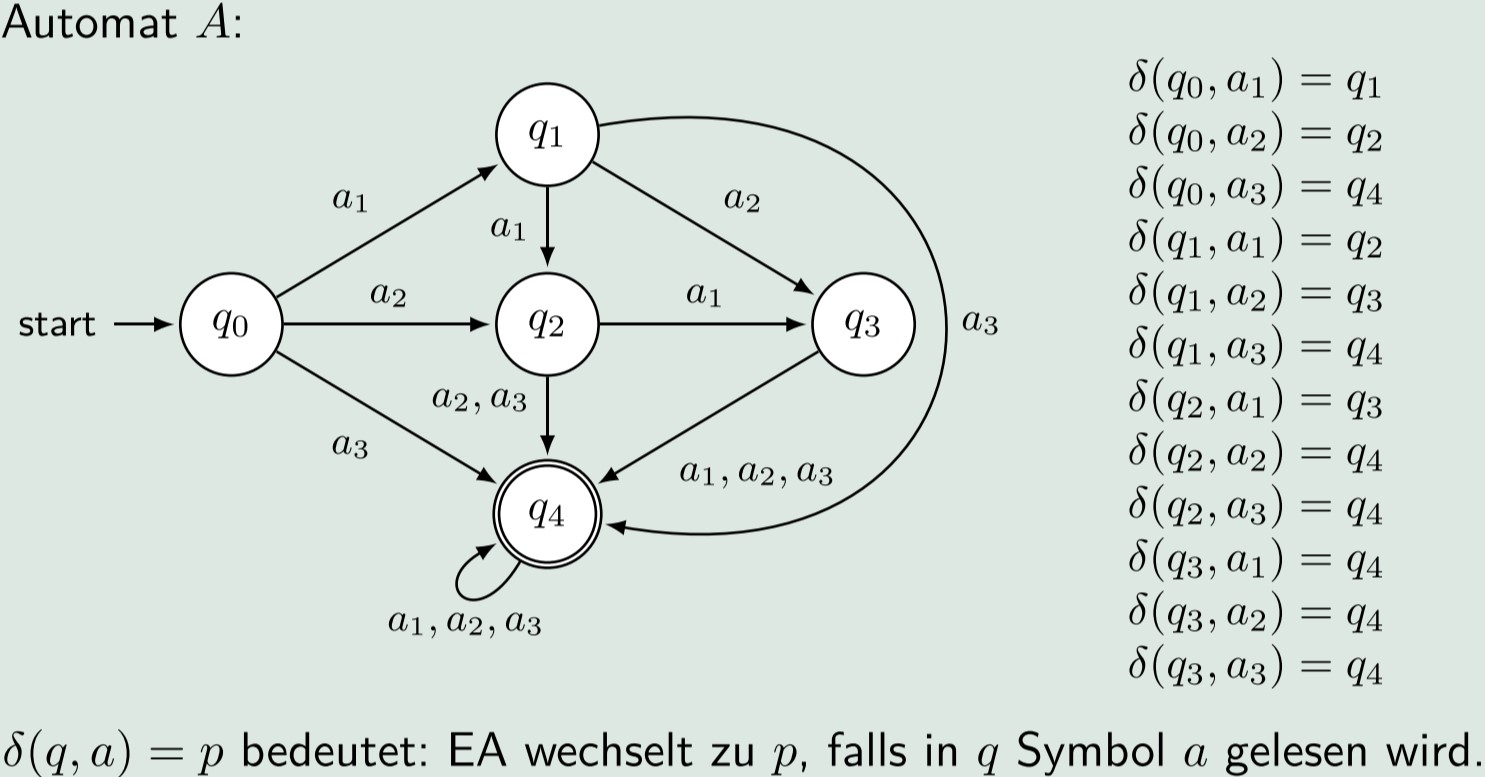
\includegraphics[scale=0.17]{endlicher-automat}

Sei $M$ ein EA. Eine \textbf{Konfiguration} von $M$ auf $\omega$ ist ein Element aus $Q \times \Sigma^*$.
\begin{itemize}
    \item Startkonfiguration von $M$ auf $\omega \Rightarrow \{ q_0, \omega \} \in \{ q_0\} \times \Sigma^*$
    \item Endkonfiguration $\Rightarrow (q_n, \varepsilon)$
\end{itemize}

Ein \textbf{Berechnungsschritt} $\vdash_M$ von $M$ \\ $(q, \omega) \vdash_M (p, x)$

Ein \textbf{Berechnung} ist eine endliche Folge von Berechnungsschritten.

$(q_a, \omega_1 \omega_2 \dots \omega_n) \vdash_M \dots \vdash_M (q_e, \omega_j \dots \omega_n) \\ \rightarrow (q_a, \omega_1 \omega_2 \dots \omega_n) \vdash_M^* (q_e, w_j \dots w_n)$

Sie startet in der Startkonfiguration $(q_0, \omega)$ und endet in der Endkonfiguration $(q_e, \varepsilon)$.
Sie ist \textbf{akzeptierend}, wenn $q_e \in F$ gilt, und \textbf{verwerfend}, falls $q_e \notin F$.

\ssect{Nichtdeterminismus}

Bei \textbf{\emph{deterministischen} endlichen Automaten} folgt jede Konfiguration \textbf{eindeutig} aus der vorhergehenden Konfiguration.

Bei \textbf{\emph{nichtdeterministischen}} endlichen Automaten können auf eine Konfiguration entweder \textbf{keine}, \textbf{genau eine} oder \textbf{mehrere} unterschiedliche Konfigurationen folgen.

\ssect{NEA}

Ein nichtdeterministischer endlicher Automat (\textbf{NEA}) ist ein Quintupel \\ $M = (Q, \Sigma, \delta, q_0, F)$

Der einzige Unterschied zum DEA besteht in der Übergangsfunktion $\delta$.
\begin{itemize}
    \item \textcolor{blue}{Übergangsfunktion $\delta$}: $Q \times \Sigma \rightarrow \mathcal{P}(Q)$
\end{itemize}
Ein $\varepsilon$-NEA erlaubt zusätzlich noch $\varepsilon$ Übergänge.

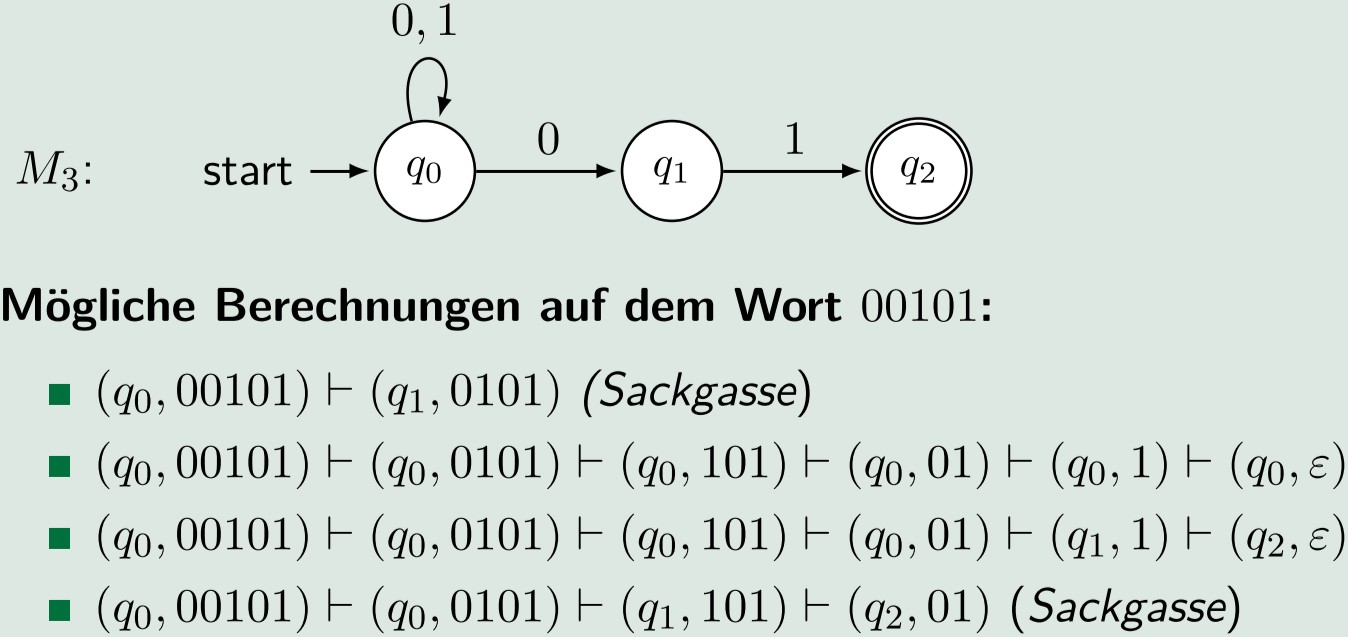
\includegraphics[scale=0.19]{nea}

DEAs, NEAs, $\varepsilon$-NEAs und RAs sind \textbf{gleichmächtig}.

\columnbreak

\ssect{Reguläre Sprachen}

Reguläre Sprachen sind durch verschiedene äquivalente Mechanismen darstellbar
\begin{itemize}
    \item Akzeptierender Mechanismus: DEA, NEA, $\varepsilon$-NEA
    \item Beschreibender Mechanismus: RA
\end{itemize}

Seien $L_1$ und $L_2$ zwei reguläre Sprachen über $\Sigma$.
Dann ist die Vereinigung ebenfalls regulär.
$L_1 \cup L_2 = \{\omega \mid \omega \in L_1 \lor \omega \in L_2\}$

Seien $L_1$ und $L_2$ zwei reguläre Sprachen über $\Sigma$.
Dann sind die \textbf{Konkatenation} $L_1 \cdot L_2 = \{ \omega = \omega_1 \omega_2 \mid \omega_1 \in L_1 \land \omega_1 \in L_2 \}$ und die \textbf{Kleenesche Hülle} \\ $L^* = \{ \omega = \omega_1 \dots \omega_n \mid \omega_i \in L$ für alle $i \in \{1, \dots, n\} \}$ auch regulär.

Sei $L$ eine reguläre Sprache über $\Sigma$.
Dann ist auch das \textbf{Komplement} $\overline{L} = \Sigma^* - L = \{ w \in \Sigma^* \mid w \notin L \}$ regulär.

% TODO: Zustandsklasse